\documentclass[aps,prl,twocolumn,superscriptaddress,showpacs,floatfix]{revtex4-1}
\usepackage[utf8x]{inputenc}
\usepackage[italian]{babel}
\usepackage{amsmath,graphicx,amsfonts}
%%%%% NEWCOMMANDS %%%%%%%%%%%%%%%%%%%%%%%%%%%%%%%%%%%%%%%%%%%%%%%%%%%%%

%%%%%%%%%%%%%%%%%%%%%%%%%%%%%%%%%%%%%%%%%%%%%%%%%%%%%%%%%%%%%%%%%%%%%%
\begin{document}
\title{Trattatello ad uso dei consumatori del sì detto \textit{G-Switch} in modalit�  multiplayer, ovvero nobile giuoco di dinamica bidimensionale in fluidi a basso numero di Reynolds}
%%%%%%%%%%%%%%%%%%%%%%%%%%%%%%%%%%%%%%%%%%%%%%%%%%%%%%%%%%%%%%%%%%%%%%
\author{G.~Bocchi}
\author{F.~Bonetti}
\author{M.~Ruggeri}
\author{V.~Tampe}
%\affiliation{New Zealand Group, Dipartimento di Fisica dell'Universit�  degli Studi
%di Milano, I-20133 Milano, Italia.}
\author{E.~Tesio}
\affiliation{New Zealand Group, Dipartimento di Fisica dell'Universit�  degli Studi
di Milano, I-20133 Milano, Italia.}
%%%%%%%%%%%%%%%%%%%%%%%%%%%%%%%%%%%%%%%%%%%%%%%%%%%%%%%%%%%%%%%%%%%%%%
\date{\today}
\begin{abstract}
Scopo del presente testo è la divulgazione, ad un livello comunque dedicato a non tutti, e bensì ai pochi, sebbene non pochissimi, che gi�  riconoscono nelle meccaniche proprie dell'attivit�  switchica un qualcosa di inerente alla propria esistenza, inutile prima e dopo la lettura dello stesso, ma densa di perchè soltanto nel mentre dell'acquisizione dei contenuti ivi presentati.
\end{abstract}
\maketitle
%%%%%%%%%%%%%%%%%%%%%%%%%%%%%%%%%%%%%%%%%%%%%%%%%%%%%%%%%%%%%%%%%%%
E' ben noto a tutti il funzionamento del giuoco, che pure riportiamo per completezza è comodit�  dell'ingroppito lettore [\onlinecite{<GF>}].\\
Dicesi \textit{G Switch} un software, originariamente in linguaggio Flash, atto a evidenziare la necessit�  di ottimizzare il codice in presenza di operazioni contemporanee da parte della macchina in esame. Scopo ludico dell'attivit�  è la conquista del traguarda da parte di un'entit�  -- scherzosamente rassomigliante a Tampe -- freneticamente movente gli arti inferiori nella folle ricerca dell'obiettivo. Per chi avesse esaurito le dinamiche relative al gioco single-player, un'ulteriore caratterizzazione del personaggio è altresì fornita; rimandiamo al superamento di questi (banali) livelli per ulteriori approfondimenti.\\
La fisica del gioco è evidente fin dai primi istanti: per quanto il nome stesso dell'attivit�  videoludica rimandi alla ben nota
\begin{equation}
G_{\mu\nu}=8\pi T_{\mu\nu}
\end{equation}
in relazione a una metrica piatta minkowskiana in due dimensioni spaziali, è chiaro ad un'analisi più approfondita che l'esistenza di tali pupattoli ludici è invece limitata ad un'universo a bassi numeri di Reynolds
\begin{equation}
R=\frac{\varrho U L}{\eta}
\end{equation}
con $\varrho$ densit�  del fluido, $U$ velocit�  dell'ominide in esame, $L$ dimensioni lineari del suddetto, e infine $\eta$ primo coefficiente di viscosit�  del mezzo. Rimarchiamo fin d'ora che la velocit�  caratteristica è funzione altamente non lineare della distanza dall'ominide dal centro di massa del sistema individuato dai corridori (eventualmente fittizi). La saturazione della variabile $U$ è ottenuta esattamente al centro di massa.

Passiamo nel seguito alla descrizione della dinamica di gioco, come sviluppata in lunghe ore di simulazioni condotte all'Universit�  degli Studi di Milano. Un Mondiale è una successione di sfide in corrispondenza biunivoca con le soluzioni (anche complesse, scemotto!) dell'equazione $z^3=1$ nel piano di Gauss, percorse per un totale di $4\pi$ con raggio unitario (si veda la Fig.~(\ref{fig:Mondiale})); a ogni livello è quindi associato un valore dell'angolo $\vartheta$, con la periodicit�  determinata in modo naturale una volta fissata la partita iniziale al valore $\vartheta=0$.
\begin{figure}
\centering
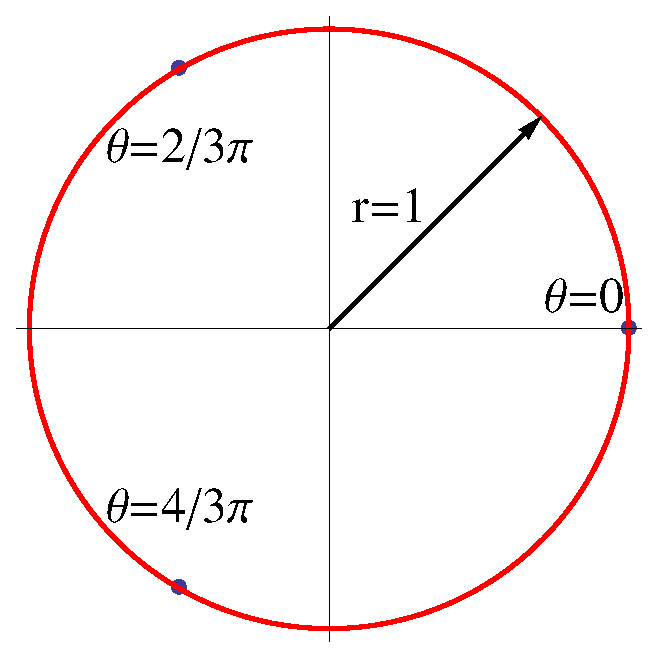
\includegraphics[scale=0.4]{Mondiale.eps}
\caption{Mundialito}
\label{fig:Mondiale}
\end{figure}
$\alpha$ protagonisti, $\alpha=1,\dots , \lfloor 2\pi\rfloor$ si sfidano ad ogni partita; $\alpha$ è fissato per ogni Mondiale. Ad $\alpha$ fissato, ogni tasto dell'insieme al più numerabile 
\begin{center}
$\mathcal A$ := \{\verb:X:, \verb:M:, $\rightarrow$, \verb:A:, \verb:Ctrl:, \verb:3:\}
\end{center}
è associato, secondo la relazione d'ordine
\[
\texttt X \succ \texttt M \succ \rightarrow \succ \texttt A \succ \texttt{Ctrl} \succ \texttt 3\;,
\]
 alle controparti umane associate biunivocamente ai pupottini corridori.\\
 A dispetto del nome che lascia sottintendere (anche correttamente, alla luce dell'interpretazione fluidodinamica prima illustrata) un'inversione del segno del campo gravitazionale al quale i pupottini sono sottoposti, l'effetto misurabile risulta unicamente in un'inversione della velocit�  nella direzione $y$. E' curioso sottolineare come l'oggetto in esame possa quindi essere in tutto equiparato ad un'esperienza di Millikan moderna: ogni pupottino possiede infatti la possibilit�  di switchare indipendentemente la propria velocit�  [\onlinecite{<Galg>}].
\section{Assiomi}
Il funzionamento principale dell'attivit�  switchica è lasciato prevalentemente all'esperienza diretta della stessa. Per i più teorici dei presenti autori ie giuocatori riportiamo tuttavia un \textit{brief resumé} che compensi l'ignoranza iniziale del lettore.\\
I pupottini sfidantisi muovono in un fluido a bassi numeri di Reynolds in 2D: la velocit�  lungo l'asse longitudinale è determinata da una funzione non lineare della variabile spaziale stessa (vedi Fig.(\ref{fig:sat})), la quale satura al valore della coordinata corrispondente al centro di massa del sistema. E' considerata \textit{uscita} la configurazione pupottica nella quale il soggetto in questione assume coordinate longitudinali negative, ovvero viene raggiunto dal fluido comovente al sistema a causa del suo ingroppimento - o di eventuali \textit{mosse} subite, si veda al proposito la sezione successiva.
\begin{figure}[!h]
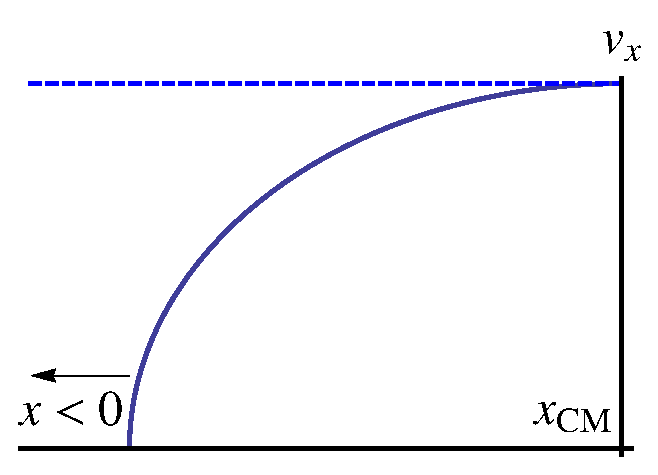
\includegraphics[scale=0.5]{sat.eps}
\caption{Rappresentazione (unitaria) qualitativa del meccanismo di saturazione della velocit�  (normalizzata) nel centro di massa del sistema fluido-pupottino. L'uscita corrisponde al raggiungimento di coordinate $x<0$.}
\label{fig:sat}
\end{figure}
La velocit�  lungo la direzione $y$ può essere switchata via software mediante la pressione di un tasto; rimarchiamo fin d'ora l'importanza del \textit{G-Switch} come primo e imperdibile esempio di software concepito per un hardware di tipo semplificato, corrispondente a un solo tasto e camionate di memoria RAM di ultima generazione.

\begin{table}[here]
\begin{center}
\begin{tabular}{||p{0.7cm}|p{0.7cm}|p{0.7cm}|p{0.7cm}|p{0.7cm}|p{0.7cm}||}
%\multicolumn{6}{c}{$\alpha\rightarrow$}\\[0.1cm]
\hline
\centering$\alpha\rightarrow$&\centering	\textbf{2}	&\centering	\textbf{3}	&\centering	\textbf{4}	&\centering	\textbf{5}	&	\hspace*{0.25cm}\textbf{6}\\
\centering $\sharp\downarrow$		&	&	&	&	&	\\
\hline
\hline

\centering \textbf{W}		&\centering	 2	&\centering	 4	&\centering 	6	&\centering 	8	& \hspace*{0.2cm}10	\\
\hline

\centering \textbf{2}		&\centering 1	&\centering	 2	&\centering  	4	&\centering 	5	&\hspace*{0.2cm}	6\\
\hline

\centering \textbf{3}		&		&\centering 	1	&\centering 	2	&\centering 	3	&\hspace*{0.2cm} 	4	\\
\hline

\centering \textbf{4}		&		&		& \centering 	1	&\centering 	2	&\hspace*{0.2cm} 	3	\\
\hline

\centering \textbf{5}		&		&		&		&\centering 	1	&\hspace*{0.2cm} 	2	\\
\hline

\centering \textbf{L}		&		&		&		&		& \hspace*{0.2cm}	1	\\
\hline
\end{tabular}
\end{center}
\caption{Punteggi corrispondenti alle diverse situazioni di giuoco multiplayer. $\alpha$ è la dimensionalit�  del Mondiale considerato, mentre $\sharp$ rappresenta la posizione raggiunta. Ai punteggi nominali va aggiunto il punteggio normalizzato a $1.00$ corrispondente al completamento del livello.}
\label{tab:punti}
\end{table}
Il completamento del livello è raggiunto grazie a una configurazione nella quale la coordinata longitudinale raggiunge forzatamente coordinata negativa; il punteggio relativo è normalizzato in unit�  naturali a $1.00$ [\onlinecite{<punti>}]. I punteggi associati alla posizione di arrivo, inversamente proporzionale alla coordinata temporale alla quale corrisponde l'uscita, è dipendente da $\alpha$ secondo lo schema riportato nella Tabella~(\ref{tab:punti}).

Ai punteggi sopra riportati è associata una struttura gruppale ereditata dall'operazione di somma sul campo reale $\mathbb{R}$; al termine del mondiale il punteggio maggiore secondo la relazione d'ordine naturale associa univocamente il vincitore del Mondiale stesso, al quale vanno quindi tributati festeggiamenti e onori. Ricordiamo che non esiste pareggio, il quale altro non è se non una mera illusione dettataci dal velo di Maya dell'imprecisione limitata a grandezze dell'ordine di $10^{-2}$.
%-----------------------%
\section{Tecnicherie, ma questo è il mestiere}

\subsection*{Blocco} Forse la più banale e semplice delle \textit{mosse} a disposizione, il blocco consiste nell'impossibilitazione al pupottin-avversario di invertire la velocit� , causando l'esaurimento del livello comobile col fluido nel mentre che il suddetto è ancora schiavo dell'ostruzione per via orizzontale. Il soggetto agente il blocco switcha quindi la velocit�  all'istante desiderato: gli obiettivi solitamente perseguiti sono l'eliminazione diretta o il rallentamento (meno pericoloso, per quanto poco maschio).
\begin{figure}[!h]
\centering
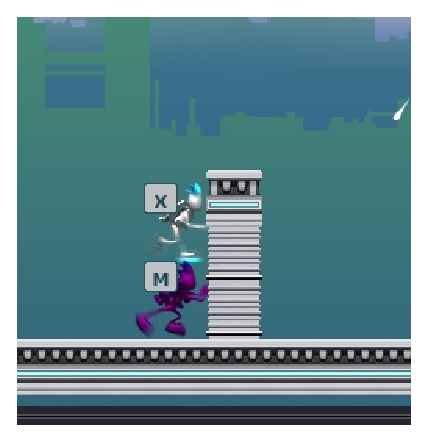
\includegraphics[scale=0.5]{blocco.eps}
\label{fig:blocco}
\caption{Vediamo in figura \texttt X che opera una configurazione di blocco sull'ingroppito \texttt M.}
\end{figure}
\subsection*{50-50} Dicesi $50-50$ la situazione nella quale due pupottini condividono la medesima posizione al momento dell'uscita dal fluido. Questo può accadere in diversi istanti della partita, e porta i pupottini in una situazione di incertezza riguardo al punteggio, dato che, considerata la maschiezza intrinseca al giuoco, il pareggio non è contemplato. La tradizionale descrizione stocastica del fenomeno è minata alle basi da recenti osservazioni, che sembrano indicare uno schema di regolarit�  basato sulla relazione d'ordine sopra citata. Ricordiamo altresì che non è dato alla sovrastuttura umana partecipante alcuna informazione oltre la seconda cifra decimale della coordinata longitunale, normalizzata, che è naturale utilizzare per descrivere il sistema.
\begin{figure}[!h]
\centering
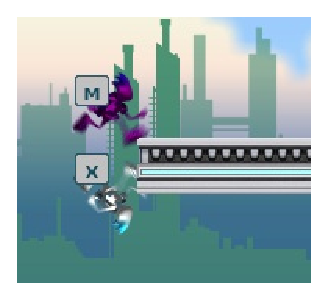
\includegraphics[scale=0.6]{50-50.eps}
\caption{Rappresentazione in real-time di una configurazione a $50-50$; osservazioni di carattere empirico danno vincente il pupottino \texttt X.}
\label{fig:50-50}
\end{figure}

\subsection*{Giova} 
La \emph{variante Giova} è una mossa utilizzata in presenza di avversari ingroppiti, e consiste in una variante a eliminazione diretta basata su uno specifico passaggio del livello corrispondente a $\vartheta=0,2\pi$. Riferiamo pertanto alla figura (\ref{fig:giova}): 
\begin{figure}[!h]
\centering
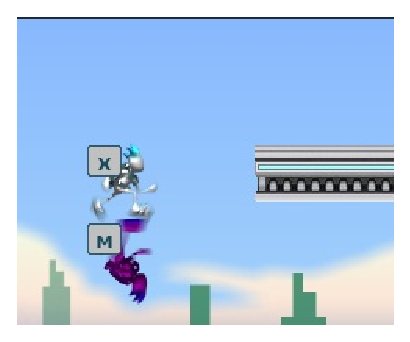
\includegraphics[scale=0.6]{giova.eps}
\caption{Un ingroppito \texttt X subisce la \emph{Giova} da parte di \texttt M. Per esaltare la didatticit�  del presente testo, in figura la sovrastuttura umana di \texttt M è identificata con l'autore stesso, per gentile concessione di egli medesimo.}
\label{fig:giova}
\end{figure}
notiamo come il pupottino  \texttt X abbia a disposizione solo un suicidio tattico per evitare che \texttt M possa proseguire nel livello successivamente all'eliminazione di \texttt X; notiamo altresì che l'eliminazione di \texttt X è comunque ineludibile.

\subsection*{Triplo} E' noto ai più che nei livelli corrispondenti a $\vartheta=...$ non è possibile il sorpasso, eccettuate ingroppitudini auto-eliminatorie, nella fase finale del livello. Più concisamente, detta $x_i$ la coordinata longitudinale associata all'$i$-esimo pupottino, la vittoria è assegnata a quest'ultimo qualora $x_i\ge x_j+\varepsilon$, $\forall j\neq i\,,\varepsilon>0$ [\onlinecite{<LI>}]. Questi più non sanno però che nel passaggio finale, il quale sembra  configurarsi appunto come il più semplice, consegnante l'agognata vittoria di tappa al pupottino con coordinata longitudinale anche solo infinitesimamente superiore, nasconde in realt�  la possibilit�  tampica di superare il pupottin-vincitore per così dire in finazza, grazie a un pericoloso e molto maschio \emph{triplo}.\begin{figure}[!h]
\centering
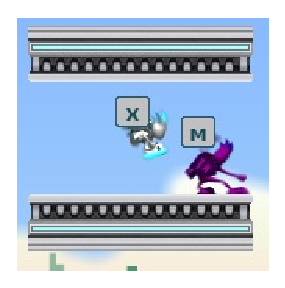
\includegraphics[scale=0.6]{triplo.eps}
\caption{Un audace \texttt X opera un \emph{triplo} ai danni di \texttt M. Sempre nell'ottica di fornire al lettore la massima e approfondita comprensione del fenomeno, il \emph{triplo} è qui effettato dal Gran Maestro, la cui fede incrollabile nell'accadimento di un triplo switch con sorpasso è tanto incrollabile e salda da comunicare in figura, unita alla più sopraffina tecnica, la feroce passione di questa circostanza.}
\label{fig:triplo}
\end{figure}
Questo è descrivibile, all'atto pratico, come una rapida successione di $N=3$ switch della velocit� , i quali permettono di entrare in configurazione di vantaggio rispetto al (gi�  cantante vittoria) pupottino avversario. Benchè questa occorrenza non si sia ancora empiricamente manifestata, è forte nei giuocatori la fede, nonchè grande e viva la speranza.

\subsection*{Trenino}
Con riferimento ai livelli $\vartheta=\tfrac{2}{3}\pi,\tfrac{2}{3}\pi+2\pi$, è possibile nei primi istanti di giuoco bloccare uno dei pupazzottoli contendenti in ambo le direzioni permesse, grazie a un eventuale accordo tra due pupattoli con coordinata $x$ maggiore. Come sempre ci riferiamo all'autoevidente situazione in Fig.~(\ref{fig:trenino}); sottolineiamo la pericolosit�  di questa \emph{mossa} soprattutto per il pupottino intermedio (nell'esempio, \texttt X), e la poca maschiezza del non operarla qualora la possibilit�  venga resa manifesta. Nel caso di mondiali ad $\alpha$ superiore è possibile operare configurazioni a trenino anche in altri livelli, sfruttando la maggior lunghezza della configurazione ottenuta; è naturalmente necessaria in questo caso una maschiezza $\sim e^\alpha$.
\begin{figure}[!h]
\centering
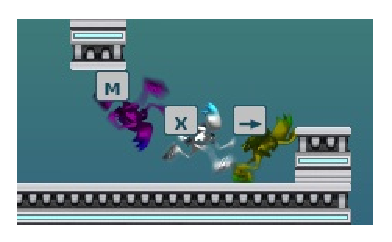
\includegraphics[scale=0.6]{trenino.eps}
\caption{Una configurazione detta \emph{a trenino}, nella quale il malcapitato \texttt M subisce l'accordo prestabilito di \texttt X e $\rightarrow$, porgendo il fianco ad una assai precoce (e cocente) eliminazione.}
\label{fig:trenino}
\end{figure}

\subsection*{Panino}
Il \emph{panino} è una variante a eliminazione o rallentamento simile al trenino, ma operata in direzione $y$. L'ingroppito pupottino intermedio è ivi bloccato per via orizzontale (così come i soggetti operanti il panino stesso), e impedito nello switchamento $y$-direzionale dai pupattolotti avversari. Come sempre, la maschiezza è tutto nell'operare questa variante, e come sempre la Fig.~(\ref{fig:panino}) vale $\ge \mathcal M=1000$ parole.\\
\begin{figure}[!h]
\centering
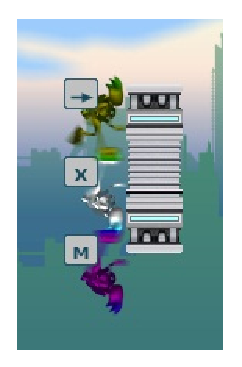
\includegraphics[scale=0.5]{panino.eps}
\caption{Un'efficace rappresentazione della configurazione \emph{a panino}, nella quale \texttt X subisce l'orribile onta dell'eliminazione da parte dei virili \texttt M e $\rightarrow$.}
\label{fig:panino}
\end{figure}
Anche questa \emph{mossa}, analogamente al \emph{trenino}, è di complessa realizzazione, in quanto sono difficilmente reperibili le distribuzioni di ostacoli adatte allo scopo. Per completezza suggeriamo infine la possibilit�  di sviuppi paninici a dimensionalit�  superiori, $\alpha>3$.
\section{Ringraziamenti}
Gli autori ringraziano sentitamente Vasco~F per aver donato loro ore di tempo perduto ma non sprecato, e ne approfittano per richiedere caldamente ulteriori sviluppi del codice, sia per la correzione di imprecisioni sia per uno sviluppo online del multiplayer.\\
Gli autori desiderano inoltre ringraziare quella meravigliosa creatura di Peter Round per averci regalato numerose frasi d'amore e tanto, tanto tempo nello switching. Ultimo, e proprio ultimo, L.~Ianni per averci permesso di affinare le più crudeli tecniche di eliminazione.

%%%%%%%%%%%%%%%%%%%%%%%%%%%%%%%%%%%%%%%%%%%
\begin{thebibliography}{100}
\bibitem{<GF>} {e.g., G.~Fatti}
\bibitem{<Galg>} {Il lettore attento noter�  subito come si stia quindi analizzando un sistema sostanzialmente classico, dato che nessuna correlazione di scambio risulta tra i vari pupottini partecipanti. Emerge inoltre in maniera naturale l'interpretazione geometrica del sistema in termini di un fibrato di gauge con gruppo di struttura abeliano
$$
U(1)^n \; ;
$$
il pupottin-multipletto viene pertanto a coincidere con una rappresentazione non-triviale del gruppo di gauge, nella quale a ciascuna componente del pupottin-multipletto si associa un numero quantico distinto da quello delle altre componenti. Al lettore più disadattato non può così sfuggire la possilit�  affascinante di considerare modelli di \emph{G Switch} gaugeato. Chiunque, infine, avr�  notato l'apprezzamento dei presenti autori per note a margine sovradimensionate, in omaggio ad un noto luminare della Meccanica Razionale di questo Ateneo.}
\bibitem{<LI>} {Una naturale eccezione, sperimentalmente verificata nella transizione di fase di prima specie $\varepsilon>0\rightarrow\varepsilon<0$, può occorrere qualora la sovrastuttura umana sia fornita da L.~Ianni.}
\bibitem{<punti>} {Ulteriori cifre significative, per quanto chimicamente utili, sono nascoste alla sovrastruttura umana.}
\end{thebibliography}


\end{document}
